\documentclass[signature=data]{physicsreport}
\usepackage{graphicx}

%%
%% User settings
%%

\classno{}
\stuno{}
\groupno{}
\stuname{}
\expdate{\expdatefmt\today}
\expname{光电效应法测定普朗克常量}

%%
%% Document body
%%

\begin{document}
% First page
% Some titles and personal information are defined in ``\maketitle''.
\maketitle

\section{实验预习指导}
\newpage

\section{原始数据记录}
% Teacher signature
\makeatletter
\physicsreport@body@signature{data}
\makeatother

\newpage

% Data process and others
\section{数据处理}

(在三个不同直径的光阑孔下分别测量对应各个光频率 $v$ 的截止电压 $U_0$,找出两者的
线性关系。用最小二乘法与作图法求出普朗克常数 $h$ 的实验值,以及与普朗克常数标准值
$h_0 = 6.626\times 10^{-34}J \cdot s$ 的相对误差。)

1. 最小二乘法:

最小二乘公式如下:
$y=kx+b,k=\frac{\bar{v}\overline{U_c}-\overline{v \cdot U_c}}{\bar{v}^2-\bar{v^2}}$


代入数据计算得到的结果如下:

当$d=2mm$时,$k=-0.3992$

当$d=4mm$时,$k=-0.3957$

当$d=6mm$时,$k=-0.3900$

又根据普朗克常数实验值和斜率的关系:$h=|k|e$,代入可得:

当$d=2mm$时,$h=6.3947\times10^{-34},E=3.49\%$

当$d=4mm$时,$h=6.3387\times10^{-34},E=4.34\%$

当$d=6mm$时,$h=6.2473\times10^{-34},E=5.72\%$

(注:$h$为普朗克常数实验值,$E$为实验误差)

2. 作图法:

用python画图如下:

\begin{figure}[H]
    \centering
    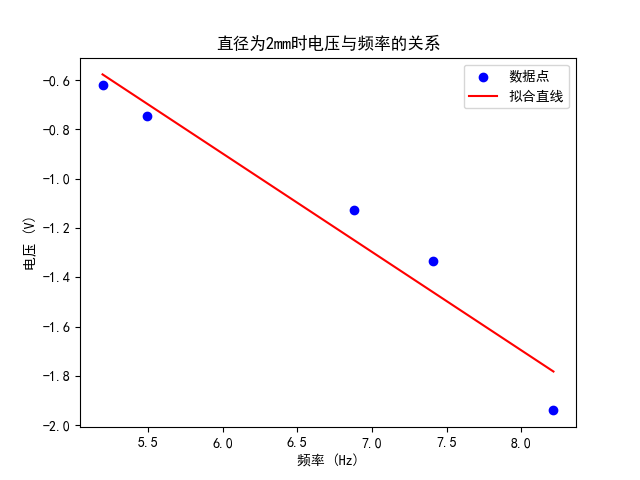
\includegraphics[width=0.8\textwidth]{images/lab13/Figure_1.png}
\end{figure}

\begin{figure}[H]
    \centering
    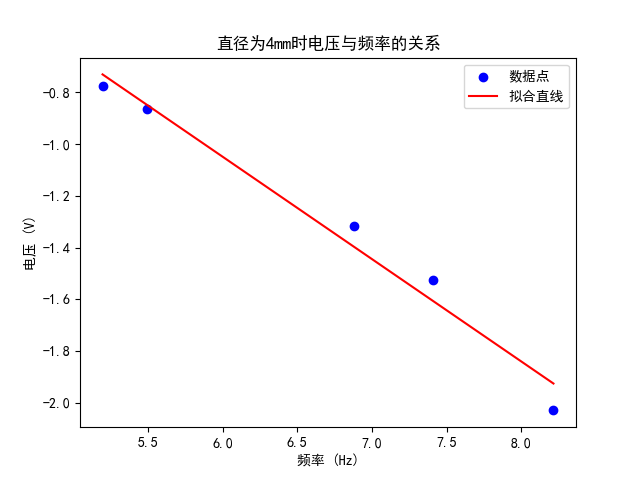
\includegraphics[width=0.8\textwidth]{images/lab13/Figure_2.png}
\end{figure}

\begin{figure}[H]
    \centering
    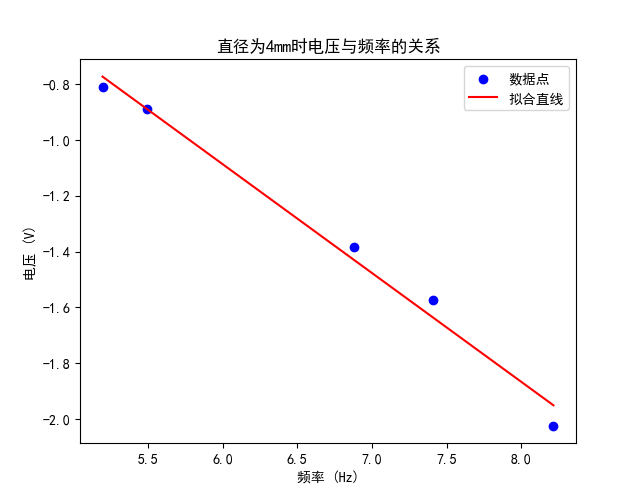
\includegraphics[width=0.8\textwidth]{images/lab13/Figure_3.png}
\end{figure}



计算得出相关结果如下:

当$d=2mm$时,$k=-0.3872,h=6.5935\times10^{-34},E=0.26\%$

当$d=4mm$时,$k=-0.3907,h=6.4757\times10^{-34},E=3.87\%$

当$d=6mm$时,$k=-0.3923,h=6.3873\times10^{-34},E=4.83\%$



\section{实验结论及现象分析}
(分析实验误差的来源,以及比较以上每种数据处理方法的优缺点)


\strong{1、误差来源:}

电压测量的精度:实验中使用的电表或电源的精度可能限制了对截止电压的精确测量。

光电管的老化或污染:光电管长时间使用后,表面污染或材料老化可能降低其性能。

环境光的干扰:实验室内的背景光可能引发光电管的额外光电流。


\strong{2、数据处理方法的优缺点:}

最小二乘法:

优点:这种方法数学严谨,能够充分利用所有数据点,减少随机误差,得到最佳拟合曲线。同时,它可以提供斜率和截距的估计值及其不确定度,有助于分析误差。

缺点:计算较为复杂,尤其是手动处理时。该方法对实验数据有一定的前提假设,例如假设误差服从正态分布。

作图法:

优点:操作简单直观,适合快速获取结果。作图可以直接展示数据点的分布,便于发现异常数据。

缺点:由于判断直线斜率时容易受到主观因素的影响,因此精确度较低。此外,作图法不易对误差和不确定度进行准确评估。



\section{讨论题}

\subsection{请解释什么是逸出功 $A$,以及怎样可以从截止电压 $U_0$ 与光频率 $v$ 两者的线性关系
中求出逸出功 $W$。}

逸出功是电子从金属表面逸出所需的最小能量。

根据光电效应公式:

$$
e U_0 = h \nu - A
$$

其中,$U_0$ 是截止电压,$h$ 是普朗克常数,$\nu$ 是入射光频率,$e$ 是电子电荷,$A$ 是逸出功。将其改写为:

$$
U_0 = \frac{h}{e} \nu - \frac{A}{e}
$$

这表明 $U_0$ 与 $\nu$ 呈线性关系,斜率为 $\frac{h}{e}$,截距为 $-\frac{A}{e}$。

通过实验测量不同频率下的截止电压作图,得到的截距可用于计算逸出功:

$$
A = -e \times \text{截距}
$$
\subsection{请讨论一下,不同金属材料的逸出功 $A$ 会否相同,并加以解释。}

不同金属材料的逸出功不会相同。这是因为逸出功与金属材料的电子结构和表面性质密切相关。具体原因如下:

1. 电子的束缚能量:不同金属中的电子被原子核束缚的强弱不同,束缚较强的金属需要更大的能量来使电子逸出,因此逸出功较大。反之,束缚较弱的金属逸出功较小。

2. 材料表面的电子密度:金属表面电子的排列和密度也会影响逸出功。高密度电子排列的金属表面通常会增加电子逸出的难度,从而增加逸出功。

3. 表面状态和纯度:即使是相同的金属,表面的氧化、污染或材料的纯度变化都会影响逸出功。例如,表面氧化层可能增大逸出功,而表面污染或缺陷可能降低逸出功。



\subsection{请讨论一下,不同金属材料的 $U_0-v$ 线性关系会否相同,并加以解释。}

不同金属材料的 \( U_0 - \nu \) (截止电压与光频率)线性关系不会相同,主要体现在截距不同,但斜率相同。原因如下:

1. 斜率相同:
光电效应公式 \( e U_0 = h \nu - A \) 中,斜率为 \( \frac{h}{e} \),其中 \( h \) 是普朗克常数,\( e \) 是电子电荷,这两个值是物理常数,与材料无关。因此,所有金属的 \( U_0 - \nu \) 关系的斜率是相同的。

2. 截距不同:
不同金属的逸出功 \( A \) 不同,公式中的截距 \( -\frac{A}{e} \) 取决于金属的逸出功。由于不同金属的逸出功 \( A \) 有差异,因此截距不同。逸出功较大的金属,其截距更负,意味着在相同频率下需要更高的光子能量才能使电子逸出。
。

\subsection{请解释什么是暗电流、本底电流、和阳极反向电流,以及它们各自出现的原因,并讨论它们各自会怎样影响“零电流法”对截止电压 $U_0$ 的测量结果。}

1. 暗电流:

暗电流是在没有光照的情况下,光电管内部产生的电流,主要由热电子或漏电流引起。

影响:使得零电流法测得的截止电压 \( U_0 \) 偏高,因为电流无法真正归零。

2. 本底电流:

本底电流由环境光引起,即使实验光源未作用时也会产生。

影响:使 \( U_0 \) 测量值偏低,因本底光叠加了额外电流。

3. 阳极反向电流:

阳极反向电流是在反向电压下产生的,由二次电子发射等原因引起的电流。

影响:使 \( U_0 \) 测量偏高,因为反向电流干扰了零点的确定。


\end{document}